\documentclass[aspectratio=169]{beamer}
\usetheme{Madrid}
\usecolortheme{default}

% Packages
\usepackage{amsmath}
\usepackage{amssymb}
\usepackage{graphicx}
\usepackage{tikz}
\usepackage{booktabs}
\usepackage{xcolor}
\usepackage{array}

% Title page information
\title[MCDM Methods]{Multi-Criteria Decision Making for Renewable Energy Planning}
\subtitle{Session 2: Methods and Techniques}
\author{Your Name}
\institute{Your Institution}
\date{\today}

% Custom colors
\definecolor{energygreen}{RGB}{34,139,34}
\definecolor{solarorange}{RGB}{255,140,0}
\definecolor{windblue}{RGB}{70,130,180}
\definecolor{methodred}{RGB}{220,20,60}

\begin{document}

% Title slide
\begin{frame}
\titlepage
\end{frame}

% Outline
\begin{frame}{Session 2 Overview}
\tableofcontents
\end{frame}

\section{Introduction to MCDM Methods}

\begin{frame}{The MCDM Methods Landscape}
\begin{columns}
\begin{column}{0.6\textwidth}
\textbf{Why do we need different methods?}
\begin{itemize}
\item Different problem characteristics
\item Varying data availability
\item Different stakeholder preferences
\item Computational complexity considerations
\end{itemize}

\vspace{0.3cm}
\textbf{Today's Focus: Four Key Methods}
\begin{enumerate}
\item \textcolor{energygreen}{\textbf{SAW}} - Simple Additive Weighting
\item \textcolor{solarorange}{\textbf{WPM}} - Weighted Product Model
\item \textcolor{windblue}{\textbf{TOPSIS}} - Technique for Order Preference by Similarity to Ideal Solution
\item \textcolor{methodred}{\textbf{AHP}} - Analytic Hierarchy Process
\end{enumerate}
\end{column}
\begin{column}{0.4\textwidth}
\begin{tikzpicture}[scale=0.8]
% Method comparison diagram
\node[rectangle, draw, fill=energygreen!20] (saw) at (0,3) {SAW};
\node[rectangle, draw, fill=solarorange!20] (wpm) at (3,3) {WPM};
\node[rectangle, draw, fill=windblue!20] (topsis) at (0,1) {TOPSIS};
\node[rectangle, draw, fill=methodred!20] (ahp) at (3,1) {AHP};

\node[ellipse, draw] (simple) at (1.5,4) {Simple};
\node[ellipse, draw] (complex) at (1.5,0) {Complex};

\draw[dashed] (simple) -- (saw);
\draw[dashed] (simple) -- (wpm);
\draw[dashed] (complex) -- (topsis);
\draw[dashed] (complex) -- (ahp);
\end{tikzpicture}
\end{column}
\end{columns}
\end{frame}

\section{Simple Additive Weighting (SAW)}

\begin{frame}{Simple Additive Weighting (SAW)}
\begin{block}{Core Concept}
Calculate weighted sum of normalized scores for each alternative
\end{block}

\textbf{Mathematical Formula:}
$$S_i = \sum_{j=1}^{n} w_j \times r_{ij}$$

Where:
\begin{itemize}
\item $S_i$ = final score for alternative $i$
\item $w_j$ = weight of criterion $j$
\item $r_{ij}$ = normalized score of alternative $i$ on criterion $j$
\item $n$ = number of criteria
\end{itemize}

\vspace{0.3cm}
\textbf{Normalization for Benefits:} $r_{ij} = \frac{x_{ij}}{\max_i(x_{ij})}$

\textbf{Normalization for Costs:} $r_{ij} = \frac{\min_i(x_{ij})}{x_{ij}}$
\end{frame}

\begin{frame}{SAW: Step-by-Step Calculation Example}
\textbf{Problem:} Choose best renewable energy for a small city

\textbf{Step 1: Decision Matrix (Raw Data)}
\begin{center}
\begin{tabular}{|l|c|c|c|}
\hline
\textbf{Alternative} & \textbf{Cost (\$/MW)} & \textbf{CO₂ (tons/MWh)} & \textbf{Reliability (\%)} \\
\hline
Solar & 1200 & 0.02 & 25 \\
Wind & 1600 & 0.01 & 35 \\
Gas & 800 & 0.35 & 85 \\
\hline
\end{tabular}
\end{center}

\textbf{Step 2: Normalize (Cost=bad, CO₂=bad, Reliability=good)}
\begin{center}
\begin{tabular}{|l|c|c|c|}
\hline
\textbf{Alternative} & \textbf{Cost} & \textbf{CO₂} & \textbf{Reliability} \\
\hline
Solar & 800/1200=0.67 & 0.01/0.02=0.50 & 25/85=0.29 \\
Wind & 800/1600=0.50 & 0.01/0.01=1.00 & 35/85=0.41 \\
Gas & 800/800=1.00 & 0.01/0.35=0.03 & 85/85=1.00 \\
\hline
\end{tabular}
\end{center>

\textbf{Step 3: Apply Weights (Cost=0.3, CO₂=0.4, Reliability=0.3)}
\textbf{Solar:} 0.67×0.3 + 0.50×0.4 + 0.29×0.3 = 0.49
\end{frame>

\begin{frame}{SAW: Complete Calculation}
\textbf{Step 4: Calculate All Scores}

\begin{center}
\begin{tabular}{|l|c|c|c|c|c|}
\hline
\textbf{Alternative} & \textbf{Cost×0.3} & \textbf{CO₂×0.4} & \textbf{Reliability×0.3} & \textbf{Total} & \textbf{Rank} \\
\hline
Solar & 0.67×0.3=0.20 & 0.50×0.4=0.20 & 0.29×0.3=0.09 & \textbf{0.49} & 2 \\
Wind & 0.50×0.3=0.15 & 1.00×0.4=0.40 & 0.41×0.3=0.12 & \textbf{0.67} & 1 \\
Gas & 1.00×0.3=0.30 & 0.03×0.4=0.01 & 1.00×0.3=0.30 & \textbf{0.61} & 3 \\
\hline
\end{tabular}
\end{center>

\textbf{Step 5: Interpret Results}
\begin{itemize}
\item \textcolor{windblue}{\textbf{Wind wins}} due to excellent environmental performance
\item \textcolor{solarorange}{\textbf{Solar second}} - balanced performance
\item \textcolor{gray}{\textbf{Gas third}} - cheap and reliable but high emissions hurt it
\end{itemize>

\vspace{0.3cm}
\textbf{Key Insight:} The 40\% weight on CO₂ emissions made environmental performance decisive!

\textcolor{red}{\textbf{What if weights were different?}} Cost=0.6, CO₂=0.2, Reliability=0.2?
\end{frame>

\begin{frame}{SAW: Advantages and Limitations}
\begin{columns}
\begin{column}{0.5\textwidth}
\textcolor{energygreen}{\textbf{Advantages:}}
\begin{itemize}
\item Simple and intuitive
\item Easy to understand and explain
\item Computationally efficient
\item Widely accepted
\item Good for initial screening
\end{itemize}

\textbf{Best for:}
\begin{itemize}
\item Simple problems
\item Clear trade-offs
\item Quantitative criteria
\item Educational purposes
\end{itemize}
\end{column}
\begin{column}{0.5\textwidth}
\textcolor{methodred}{\textbf{Limitations:}}
\begin{itemize}
\item Assumes criteria independence
\item Linear compensation
\item Sensitive to normalization
\item May not capture complex preferences
\item Rank reversal possible
\end{itemize}

\textbf{Not ideal for:}
\begin{itemize}
\item Interdependent criteria
\item Non-linear preferences
\item Qualitative assessments
\item Complex stakeholder structures
\end{itemize}
\end{column}
\end{columns}
\end{frame}

\section{Weighted Product Model (WPM)}

\begin{frame}{Weighted Product Model (WPM)}
\begin{block}{Core Concept}
Uses pairwise comparisons with ratio-based calculations to rank alternatives
\end{block}

\textbf{Mathematical Formula (Pairwise Comparison):}
$$P(A_k/A_l) = \prod_{j=1}^{n} \left(\frac{a_{kj}}{a_{lj}}\right)^{w_j}$$

\textbf{Alternative Formula (Absolute Product):}
$$P(A_k) = \prod_{j=1}^{n} (a_{kj})^{w_j}$$

Where:
\begin{itemize}
\item $P(A_k/A_l)$ = preference of alternative $k$ over $l$
\item $a_{kj}$ = value of alternative $k$ for criterion $j$
\item $w_j$ = weight of criterion $j$
\end{itemize}

\textbf{Key Advantage:} Dimensionless analysis - no unit conversion needed!
\end{frame}

\begin{frame}{WPM: The Dimensionless Advantage}
\textbf{Problem with SAW:} "Adding apples and oranges"
\begin{itemize}
\item Cost (\$) + Efficiency (\%) + Emissions (tons CO₂)
\item Different units make comparison difficult
\item Normalization affects results
\end{itemize}

\vspace{0.3cm}
\textbf{WPM Solution:} Uses ratios and multiplication
\begin{itemize}
\item Ratios are dimensionless
\item No normalization required
\item More stable results
\end{itemize}

\vspace{0.3cm}
\textbf{Example: Solar vs Wind (Same data as SAW)}
\begin{center}
\begin{tabular}{|l|c|c|c|}
\hline
& \textbf{Cost (\$/MW)} & \textbf{CO₂ (tons/MWh)} & \textbf{Reliability (\%)} \\
\hline
Solar & 1200 & 0.02 & 25 \\
Wind & 1600 & 0.01 & 35 \\
\hline
\end{tabular}
\end{center}

$$P(\text{Solar}/\text{Wind}) = \left(\frac{1600}{1200}\right)^{0.3} \times \left(\frac{0.01}{0.02}\right)^{0.4} \times \left(\frac{25}{35}\right)^{0.3}$$
$$= (1.33)^{0.3} \times (0.5)^{0.4} \times (0.71)^{0.3} = 0.82$$

Since $P(\text{Solar}/\text{Wind}) < 1$, \textcolor{windblue}{\textbf{Wind is preferred}}

\textbf{Note:} For costs, we use reciprocal ratios (higher cost = worse)
\end{frame>

\begin{frame}{WPM: Complete Analysis}
\textbf{All Pairwise Comparisons (Weights: Cost=0.3, CO₂=0.4, Reliability=0.3)}

\begin{center}
\begin{tabular}{|l|c|c|c|}
\hline
\textbf{Comparison} & \textbf{P(A/B)} & \textbf{Result} & \textbf{Preferred} \\
\hline
Solar vs Wind & 0.82 & < 1 & Wind \\
Solar vs Gas & 0.45 & < 1 & Gas \\
Wind vs Gas & 0.55 & < 1 & Gas \\
\hline
\end{tabular}
\end{center>

\textbf{Ranking Logic:}
\begin{itemize}
\item Gas beats both Solar and Wind → \textbf{Gas = 1st}
\item Wind beats Solar → \textbf{Wind = 2nd}
\item Solar loses to both → \textbf{Solar = 3rd}
\end{itemize>

\vspace{0.3cm}
\textbf{Final WPM Ranking:} Gas > Wind > Solar

\textcolor{red}{\textbf{Different from SAW!}} (SAW: Wind > Solar > Gas)

\textbf{Why?} WPM's multiplicative nature amplifies Gas's reliability advantage
\end{frame>

\begin{frame}{WPM: Advantages and Applications}
\begin{columns}
\begin{column}{0.5\textwidth}
\textcolor{energygreen}{\textbf{Advantages:}}
\begin{itemize}
\item Dimensionless analysis
\item No normalization needed
\item Handles different units well
\item More stable than SAW
\item Good for multiplicative relationships
\end{itemize}

\textbf{Renewable Energy Applications:}
\begin{itemize}
\item Technology comparison
\item Site selection
\item Investment decisions
\item Policy evaluation
\end{itemize}
\end{column}
\begin{column}{0.5\textwidth}
\textcolor{methodred}{\textbf{Limitations:}}
\begin{itemize}
\item More complex calculations
\item Requires positive values
\item Less intuitive than SAW
\item Multiplicative compensation
\item Sensitive to extreme values
\end{itemize}

\textbf{Considerations:}
\begin{itemize}
\item Handle zero values carefully
\item Cost criteria need reciprocals
\item Geometric interpretation
\item Logarithmic transformations
\end{itemize}
\end{column}
\end{columns}
\end{frame}

\section{TOPSIS Method}

\begin{frame}{TOPSIS: Technique for Order Preference by Similarity to Ideal Solution}
\begin{block}{Core Concept}
Rank alternatives based on their distance from ideal and anti-ideal solutions
\end{block}

\textbf{Key Steps:}
\begin{enumerate}
\item Normalize decision matrix: $r_{ij} = \frac{x_{ij}}{\sqrt{\sum_{k=1}^{m} x_{kj}^2}}$
\item Create weighted matrix: $t_{ij} = r_{ij} \times w_j$
\item Determine best ($A_b$) and worst ($A_w$) alternatives
\item Calculate distances: $d_{ib} = \sqrt{\sum_{j=1}^{n} (t_{ij} - t_{bj})^2}$
\item Calculate similarity: $s_{iw} = \frac{d_{iw}}{d_{iw} + d_{ib}}$
\end{enumerate}

\textbf{Interpretation:} Higher $s_{iw}$ means better alternative (closer to ideal, farther from anti-ideal)
\end{frame>

\begin{frame}{TOPSIS: Visual Interpretation}
\begin{center}
\begin{tikzpicture}[scale=1.2]
% Coordinate system
\draw[->] (0,0) -- (5,0) node[right] {Criterion 1};
\draw[->] (0,0) -- (0,4) node[above] {Criterion 2};

% Ideal and anti-ideal points
\node[circle, fill=energygreen, label=above:$A_b$ (Best)] (ideal) at (4,3.5) {};
\node[circle, fill=methodred, label=below:$A_w$ (Worst)] (antiideal) at (0.5,0.5) {};

% Alternatives
\node[square, fill=solarorange, label=right:Solar] (solar) at (3,2.5) {};
\node[square, fill=windblue, label=right:Wind] (wind) at (2.5,3) {};
\node[square, fill=gray, label=right:Coal] (coal) at (1,1) {};

% Distance lines
\draw[dashed, energygreen] (solar) -- (ideal);
\draw[dashed, methodred] (solar) -- (antiideal);
\draw[dashed, energygreen] (wind) -- (ideal);
\draw[dashed, methodred] (wind) -- (antiideal);

% Labels
\node at (2.5,0.3) {$d_{ib}$ (distance to best)};
\node at (1.5,1.8) {$d_{iw}$ (distance to worst)};
\end{tikzpicture}
\end{center}

\textbf{TOPSIS Logic:} Best alternative is closest to ideal and farthest from anti-ideal
\end{frame}

\begin{frame}{TOPSIS: Advantages and Applications}
\begin{columns}
\begin{column}{0.5\textwidth}
\textcolor{energygreen}{\textbf{Advantages:}}
\begin{itemize}
\item Considers both best and worst scenarios
\item Handles multiple criteria well
\item Intuitive geometric interpretation
\item Robust to outliers
\item Good discrimination between alternatives
\end{itemize}

\textbf{Energy Applications:}
\begin{itemize}
\item Renewable energy ranking
\item Site selection
\item Technology assessment
\item Sustainability evaluation
\end{itemize}
\end{column}
\begin{column}{0.5\textwidth}
\textcolor{methodred}{\textbf{Limitations:}}
\begin{itemize}
\item Requires quantitative data
\item Euclidean distance assumption
\item May not reflect true preferences
\item Sensitive to criteria selection
\item Complex for stakeholders to understand
\end{itemize}

\textbf{Best Practices:}
\begin{itemize}
\item Validate ideal/anti-ideal solutions
\item Consider alternative distance metrics
\item Perform sensitivity analysis
\item Combine with stakeholder input
\end{itemize}
\end{column>
\end{columns}
\end{frame}

\section{Analytic Hierarchy Process (AHP)}

\begin{frame}{Analytic Hierarchy Process (AHP)}
\begin{block}{Core Concept}
Structures complex decisions into hierarchies and uses pairwise comparisons to derive priorities
\end{block>

\textbf{AHP Hierarchy Structure:}
\begin{center}
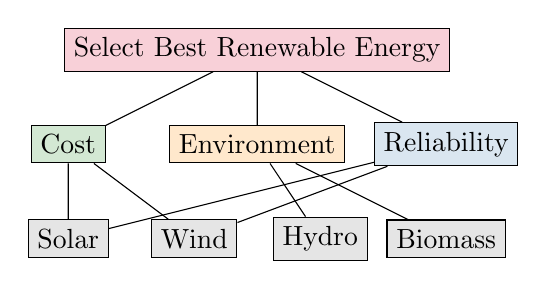
\begin{tikzpicture}[scale=0.8]
% Goal level
\node[rectangle, draw, fill=methodred!20] (goal) at (4,4) {Select Best Renewable Energy};

% Criteria level
\node[rectangle, draw, fill=energygreen!20] (cost) at (1,2.5) {Cost};
\node[rectangle, draw, fill=solarorange!20] (env) at (4,2.5) {Environment};
\node[rectangle, draw, fill=windblue!20] (rel) at (7,2.5) {Reliability};

% Alternatives level
\node[rectangle, draw, fill=gray!20] (solar) at (1,1) {Solar};
\node[rectangle, draw, fill=gray!20] (wind) at (3,1) {Wind};
\node[rectangle, draw, fill=gray!20] (hydro) at (5,1) {Hydro};
\node[rectangle, draw, fill=gray!20] (bio) at (7,1) {Biomass};

% Connections
\draw (goal) -- (cost);
\draw (goal) -- (env);
\draw (goal) -- (rel);

\draw (cost) -- (solar);
\draw (cost) -- (wind);
\draw (env) -- (hydro);
\draw (env) -- (bio);
\draw (rel) -- (solar);
\draw (rel) -- (wind);
\end{tikzpicture}
\end{center}
\end{frame}

\begin{frame}{AHP: Pairwise Comparison Process}
\textbf{Saaty's 1-9 Scale:}
\begin{center}
\small
\begin{tabular}{|c|l|}
\hline
\textbf{Intensity} & \textbf{Definition} \\
\hline
1 & Equal importance \\
3 & Moderate importance \\
5 & Strong importance \\
7 & Very strong importance \\
9 & Extreme importance \\
2,4,6,8 & Intermediate values \\
\hline
\end{tabular}
\end{center>

\textbf{Example: Criteria Comparison Matrix}
\begin{center}
\begin{tabular}{|l|c|c|c|}
\hline
& \textbf{Cost} & \textbf{Environment} & \textbf{Reliability} \\
\hline
\textbf{Cost} & 1 & 1/3 & 2 \\
\textbf{Environment} & 3 & 1 & 4 \\
\textbf{Reliability} & 1/2 & 1/4 & 1 \\
\hline
\end{tabular}
\end{center>

\textbf{Interpretation:} Environment is 3 times more important than Cost
\end{frame>

\begin{frame}{AHP: Consistency and Final Synthesis}
\textbf{Consistency Check:}
$$CR = \frac{CI}{RI} = \frac{\lambda_{max} - n}{(n-1) \times RI}$$

Where $CR < 0.1$ indicates acceptable consistency

\vspace{0.3cm}
\textbf{Final Synthesis:}
$$S_i = \sum_{j=1}^{n} w_j \times w_{ij}$$

Where:
\begin{itemize}
\item $S_i$ = final score for alternative $i$
\item $w_j$ = weight of criterion $j$
\item $w_{ij}$ = local weight of alternative $i$ under criterion $j$
\end{itemize}

\vspace{0.3cm}
\textbf{AHP Advantages:}
\begin{itemize}
\item Handles qualitative criteria
\item Captures stakeholder preferences
\item Provides consistency checks
\item Hierarchical structure clarity
\end{itemize}
\end{frame>

\section{Method Comparison and Selection}

\begin{frame}{When to Use Which Method?}
\begin{center}
\small
\begin{tabular}{|l|c|c|c|c|}
\hline
\textbf{Characteristic} & \textbf{SAW} & \textbf{WPM} & \textbf{TOPSIS} & \textbf{AHP} \\
\hline
Simplicity & ★★★ & ★★ & ★★ & ★ \\
Data Requirements & Low & Low & Medium & High \\
Stakeholder Input & Limited & Limited & Medium & High \\
Qualitative Criteria & Poor & Poor & Good & Excellent \\
Consistency Checks & No & No & No & Yes \\
Computational Complexity & Low & Low & Medium & High \\
\hline
\end{tabular}
\end{center>

\vspace{0.3cm}
\textbf{Selection Guidelines:}
\begin{itemize}
\item \textbf{SAW:} Simple problems, quantitative criteria, educational purposes
\item \textbf{WPM:} Mixed units, multiplicative relationships, dimensionless analysis
\item \textbf{TOPSIS:} Multiple quantitative criteria, clear ideal solutions
\item \textbf{AHP:} Complex hierarchies, qualitative criteria, stakeholder involvement
\end{itemize>
\end{frame>

\section{Case Study Application}

\begin{frame}{Case Study: Rural India Solar Project - Method Comparison}
\textbf{Problem:} Select best electrification option for rural community

\begin{center}
\small
\begin{tabular}{|l|c|c|c|c|}
\hline
\textbf{Method} & \textbf{1st Choice} & \textbf{2nd Choice} & \textbf{3rd Choice} & \textbf{4th Choice} \\
\hline
SAW & Solar Microgrid & Solar Home & Grid Extension & Diesel \\
WPM & Solar Microgrid & Solar Home & Grid Extension & Diesel \\
TOPSIS & Solar Microgrid & Grid Extension & Solar Home & Diesel \\
AHP & Solar Home & Solar Microgrid & Grid Extension & Diesel \\
\hline
\end{tabular}
\end{center>

\textbf{Key Insights:}
\begin{itemize}
\item All methods agree: Diesel generator is worst option
\item Solar solutions consistently rank in top 2
\item AHP gives slightly different ranking due to stakeholder preferences
\item Grid extension ranking varies by method
\end{itemize>

\textbf{Recommendation:} Solar microgrid with sensitivity analysis on key assumptions
\end{frame>

\begin{frame}{Session 2 Summary}
\textbf{Key Takeaways:}
\begin{enumerate}
\item Different MCDM methods suit different problem types
\item SAW: Simple and intuitive, good for initial analysis
\item WPM: Dimensionless, handles mixed units well
\item TOPSIS: Considers ideal solutions, robust ranking
\item AHP: Hierarchical structure, stakeholder preferences
\end{enumerate>

\vspace{0.3cm}
\textbf{Method Selection Depends On:}
\begin{itemize}
\item Data availability and quality
\item Stakeholder involvement needs
\item Problem complexity
\item Time and resource constraints
\end{itemize>

\vspace{0.3cm}
\textbf{Next Session:} Advanced applications, implementation strategies, and software tools

\begin{center}
\textcolor{energygreen}{\Large Questions?}
\end{center>
\end{frame>

\end{document>
